%%%%%%%%%%%%%%%%%%%%%%%%%%%%%%%%%%%%%%%%%
% Beamer Presentation
% LaTeX Template
% Version 2.0 (March 8, 2022)
%
% This template originates from:
% https://www.LaTeXTemplates.com
%
% Author:
% Vel (vel@latextemplates.com)
%
% License:
% CC BY-NC-SA 4.0 (https://creativecommons.org/licenses/by-nc-sa/4.0/)
%
%%%%%%%%%%%%%%%%%%%%%%%%%%%%%%%%%%%%%%%%%

%----------------------------------------------------------------------------------------
%	PACKAGES AND OTHER DOCUMENT CONFIGURATIONS
%----------------------------------------------------------------------------------------

\documentclass[
	11pt, compress% Set the default font size, options include: 8pt, 9pt, 10pt, 11pt, 12pt, 14pt, 17pt, 20pt
	%t, % Uncomment to vertically align all slide content to the top of the slide, rather than the default centered
	%aspectratio=169, % Uncomment to set the aspect ratio to a 16:9 ratio which matches the aspect ratio of 1080p and 4K screens and projectors
]{beamer}

\graphicspath{{Images/}{./}} % Specifies where to look for included images (trailing slash required)

\usepackage{booktabs} % Allows the use of \toprule, \midrule and \bottomrule for better rules in tables
\usepackage{wrapfig}


%----------------------------------------------------------------------------------------
%	SELECT LAYOUT THEME
%----------------------------------------------------------------------------------------

% Beamer comes with a number of default layout themes which change the colors and layouts of slides. Below is a list of all themes available, uncomment each in turn to see what they look like.

%\usetheme{default}
%\usetheme{AnnArbor}
%\usetheme{Antibes}
%\usetheme{Bergen}
%\usetheme{Berkeley}
\usetheme{Berlin}
%\usetheme{Boadilla}
%\usetheme{CambridgeUS}
%\usetheme{Copenhagen}
%\usetheme{Darmstadt}
%\usetheme{Dresden}
%\usetheme{Frankfurt}
%\usetheme{Goettingen}
%\usetheme{Hannover}
%\usetheme{Ilmenau}
%\usetheme{JuanLesPins}
%\usetheme{Luebeck}
%\usetheme{Madrid}
%\usetheme{Malmoe}
%\usetheme{Marburg}
%\usetheme{Montpellier}
%\usetheme{PaloAlto}
%\usetheme{Pittsburgh}
%\usetheme{Rochester}
%\usetheme{Singapore}
%\usetheme{Szeged}
%\usetheme{Warsaw}


%----------------------------------------------------------------------------------------
%	SELECT FONT THEME & FONTS
%----------------------------------------------------------------------------------------

% Beamer comes with several font themes to easily change the fonts used in various parts of the presentation. Review the comments beside each one to decide if you would like to use it. Note that additional options can be specified for several of these font themes, consult the beamer documentation for more information.

\usefonttheme{default} % Typeset using the default sans serif font
%\usefonttheme{serif} % Typeset using the default serif font (make sure a sans font isn't being set as the default font if you use this option!)
%\usefonttheme{structurebold} % Typeset important structure text (titles, headlines, footlines, sidebar, etc) in bold
%\usefonttheme{structureitalicserif} % Typeset important structure text (titles, headlines, footlines, sidebar, etc) in italic serif
%\usefonttheme{structuresmallcapsserif} % Typeset important structure text (titles, headlines, footlines, sidebar, etc) in small caps serif

%------------------------------------------------

%\usepackage{mathptmx} % Use the Times font for serif text
\usepackage{palatino} % Use the Palatino font for serif text

%\usepackage{helvet} % Use the Helvetica font for sans serif text
\usepackage[default]{opensans} % Use the Open Sans font for sans serif text
%\usepackage[default]{FiraSans} % Use the Fira Sans font for sans serif text
%\usepackage[default]{lato} % Use the Lato font for sans serif text
\expandafter\def\expandafter\insertshorttitle\expandafter{%
  \insertshorttitle\hfill%
  \insertframenumber\,/\,\inserttotalframenumber}
%----------------------------------------------------------------------------------------
%	SELECT INNER THEME
%----------------------------------------------------------------------------------------

% Inner themes change the styling of internal slide elements, for example: bullet points, blocks, bibliography entries, title pages, theorems, etc. Uncomment each theme in turn to see what changes it makes to your presentation.

%\useinnertheme{default}
%\useinnertheme{circles}
%\useinnertheme{rectangles}
\useinnertheme{rounded}
%\useinnertheme{inmargin}

\setbeamertemplate{caption}{\raggedright\insertcaption\par}

%----------------------------------------------------------------------------------------
%	SELECT OUTER THEME
%----------------------------------------------------------------------------------------

% Outer themes change the overall layout of slides, such as: header and footer lines, sidebars and slide titles. Uncomment each theme in turn to see what changes it makes to your presentation.

%\useoutertheme{default}
\useoutertheme{infolines}
%\useoutertheme{miniframes}
%\useoutertheme{smoothbars}
%\useoutertheme{sidebar}
%\useoutertheme{split}
%\useoutertheme{shadow}
%\useoutertheme{tree}
%\useoutertheme{smoothtree}

%\setbeamertemplate{footline} % Uncomment this line to remove the footer line in all slides
%\setbeamertemplate{footline}[page number] % Uncomment this line to replace the footer line in all slides with a simple slide count

%\setbeamertemplate{navigation symbols}{} % Uncomment this line to remove the navigation symbols from the bottom of all slides

%----------------------------------------------------------------------------------------
%	PRESENTATION INFORMATION
%----------------------------------------------------------------------------------------

\title[]{Ethical implications of AI-generated images}% The short title in the optional parameter appears at the bottom of every slide, the full title in the main parameter is only on the title page


%\subtitle{Optional Subtitle} % Presentation subtitle, remove this command if a subtitle isn't required

\author[]{Manuel Muehlberger \inst{1} \and Sofia Kaltwasser \inst{2}}
\institute[]{\inst{1} TU Munich \and %
                      \inst{2} University of Potsdam}

%\textit{james@LaTeXTemplates.com}} % Your institution, the optional parameter can be used for the institution shorthand and will appear on the bottom of every slide after author names, while the required parameter is used on the title slide and can include your email address or additional information on separate lines

\date{Ethik 4 Nerds \\ \smallskip 08.03.2023} % Presentation date or conference/meeting name, the optional parameter can contain a shortened version to appear on the bottom of every slide, while the required parameter value is output to the title slide
\titlegraphic{
\includegraphics[scale=0.04]{Images/logos.png}}
%----------------------------------------------------------------------------------------

\begin{document}

%----------------------------------------------------------------------------------------
%	TITLE SLIDE
%----------------------------------------------------------------------------------------

\begin{frame}[noframenumbering]
	\titlepage % Output the title slide, automatically created using the text entered in the PRESENTATION INFORMATION block above
\end{frame}

%----------------------------------------------------------------------------------------
%	TABLE OF CONTENTS SLIDE
%----------------------------------------------------------------------------------------

% The table of contents outputs the sections and subsections that appear in your presentation, specified with the standard \section and \subsection commands. You may either display all sections and subsections on one slide with \tableofcontents, or display each section at a time on subsequent slides with \tableofcontents[pausesections]. The latter is useful if you want to step through each section and mention what you will discuss.

\begin{frame}[noframenumbering]
	\frametitle{Presentation Overview} % Slide title, remove this command for no title
	\tableofcontents % Output the table of contents (all sections on one slide)
	%\tableofcontents[pausesections] % Output the table of contents (break sections up across separate slides)
\end{frame}

%----------------------------------------------------------------------------------------
%	PRESENTATION BODY SLIDES
%----------------------------------------------------------------------------------------

\section{Introduction} 

\begin{frame}
	\frametitle{AI-generated images}
	\begin{itemize}
		\item Significant advancements in recent years
		\item Realistic and high-quality images $\rightarrow$ almost indistinguishable from human-created images
		\item example Dall-E 2 by OpenAI \cite{DallE}
	\end{itemize}
\end{frame}


\begin{frame}
	\frametitle{Dall-E 2 generated images examples}
	\begin{columns}[c] 
		\begin{column}{0.5\textwidth} % Left column width
			\begin{figure}
				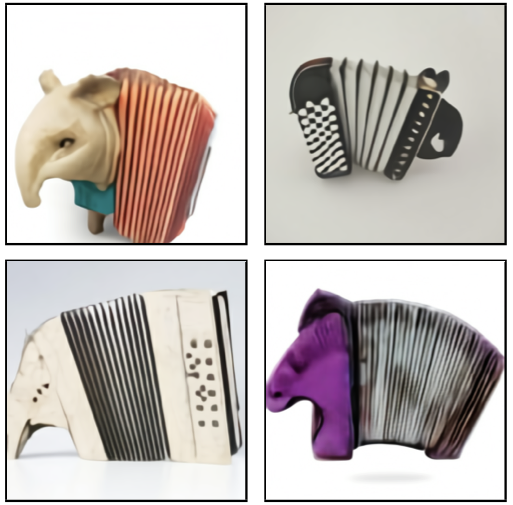
\includegraphics[width=0.95\linewidth]{Images/exampleTapir.png}
				\caption{(a) A tapir with the texture of an accordion \cite{DBLP:journals/corr/abs-2102-12092}}
			\end{figure}
		\end{column}
		\begin{column}{0.5\textwidth} % Right column width
			\begin{figure}
				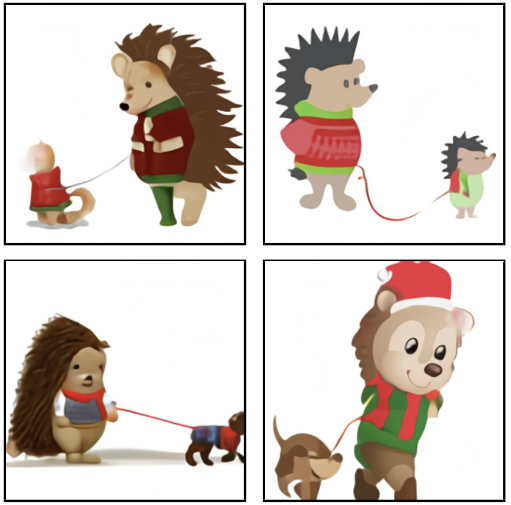
\includegraphics[width=0.95\linewidth]{Images/exampleHedgehog.png}
				\caption{(b) Illustration of a baby hedgehog in a christmas sweater walking a dog \cite{DBLP:journals/corr/abs-2102-12092}} 
			\end{figure}
		\end{column}
	\end{columns}
\end{frame}


\section{Technical}

\begin{frame}
	\frametitle{High level abstraction of image generation process of DALL-E 2}
	\begin{figure}
		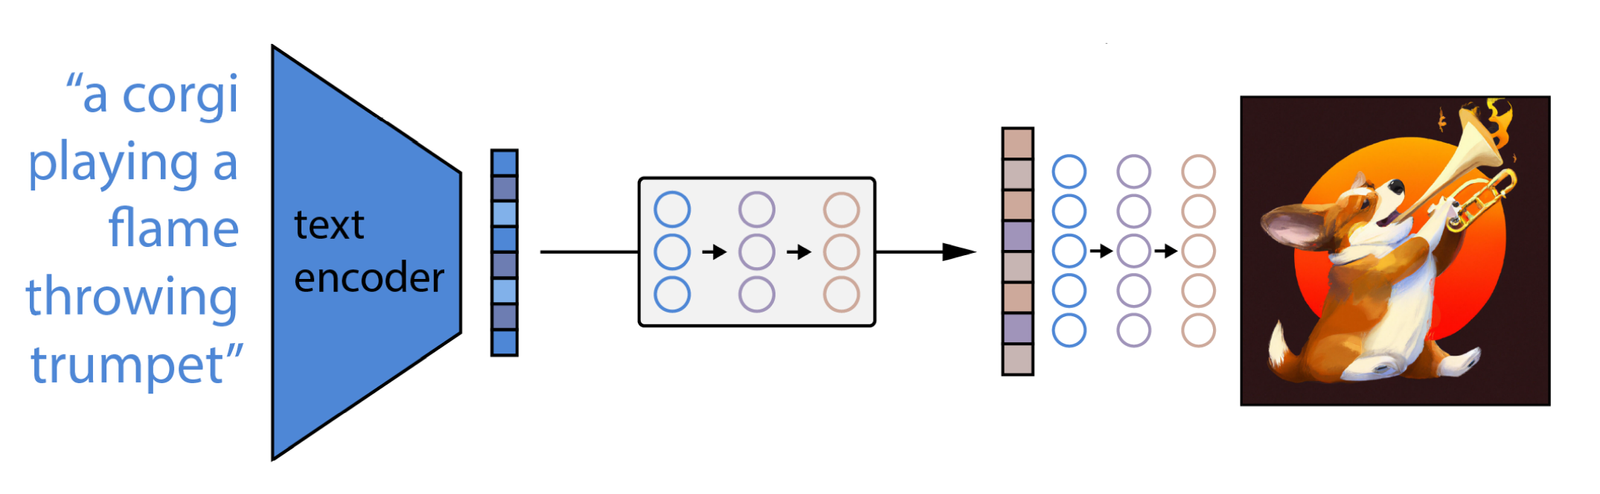
\includegraphics[width=0.85\linewidth]{Images/highLevel.png}
		\caption{High-level overview of operating principle of DallE-2 [modified from \cite{https://doi.org/10.48550/arxiv.2204.06125}]}
	\end{figure}
\end{frame}

\begin{frame}
	\frametitle{Contrastive Language-Image Pre-training (CLIP)}
	
	link between textual semantics and their visual representations
	good explanation: 
	https://www.assemblyai.com/blog/how-dall-e-2-actually-works/
\end{frame}


\section{Ethical Considerations}
\begin{frame}
\begin{center}
	\frametitle{Picture-Perfect or Ethically Problematic?}
	\huge Let's look at some problems
\end{center}
\end{frame}

% Make this short
\begin{frame}
	\frametitle{First of all: It's not all bad...}
	\begin{itemize}
		\setlength\itemsep{2em}
		\item Efficiency and Sacalability
		\item Cost-Effectiveness
		\item No specialized skills required to use
	\end{itemize}
\end{frame}

\begin{frame}
	% - Artists taking credit for AI-generated content
	% 	-> https://www.nytimes.com/2022/09/02/technology/ai-artificial-intelligence-artists.html
	%	-> can substantially harm / destroy confidence in the Art community
	%	-> cheating in games <--> cheating in art-contests
		\frametitle{Artists taking credit for AI-generated content}
		\begin{figure}
			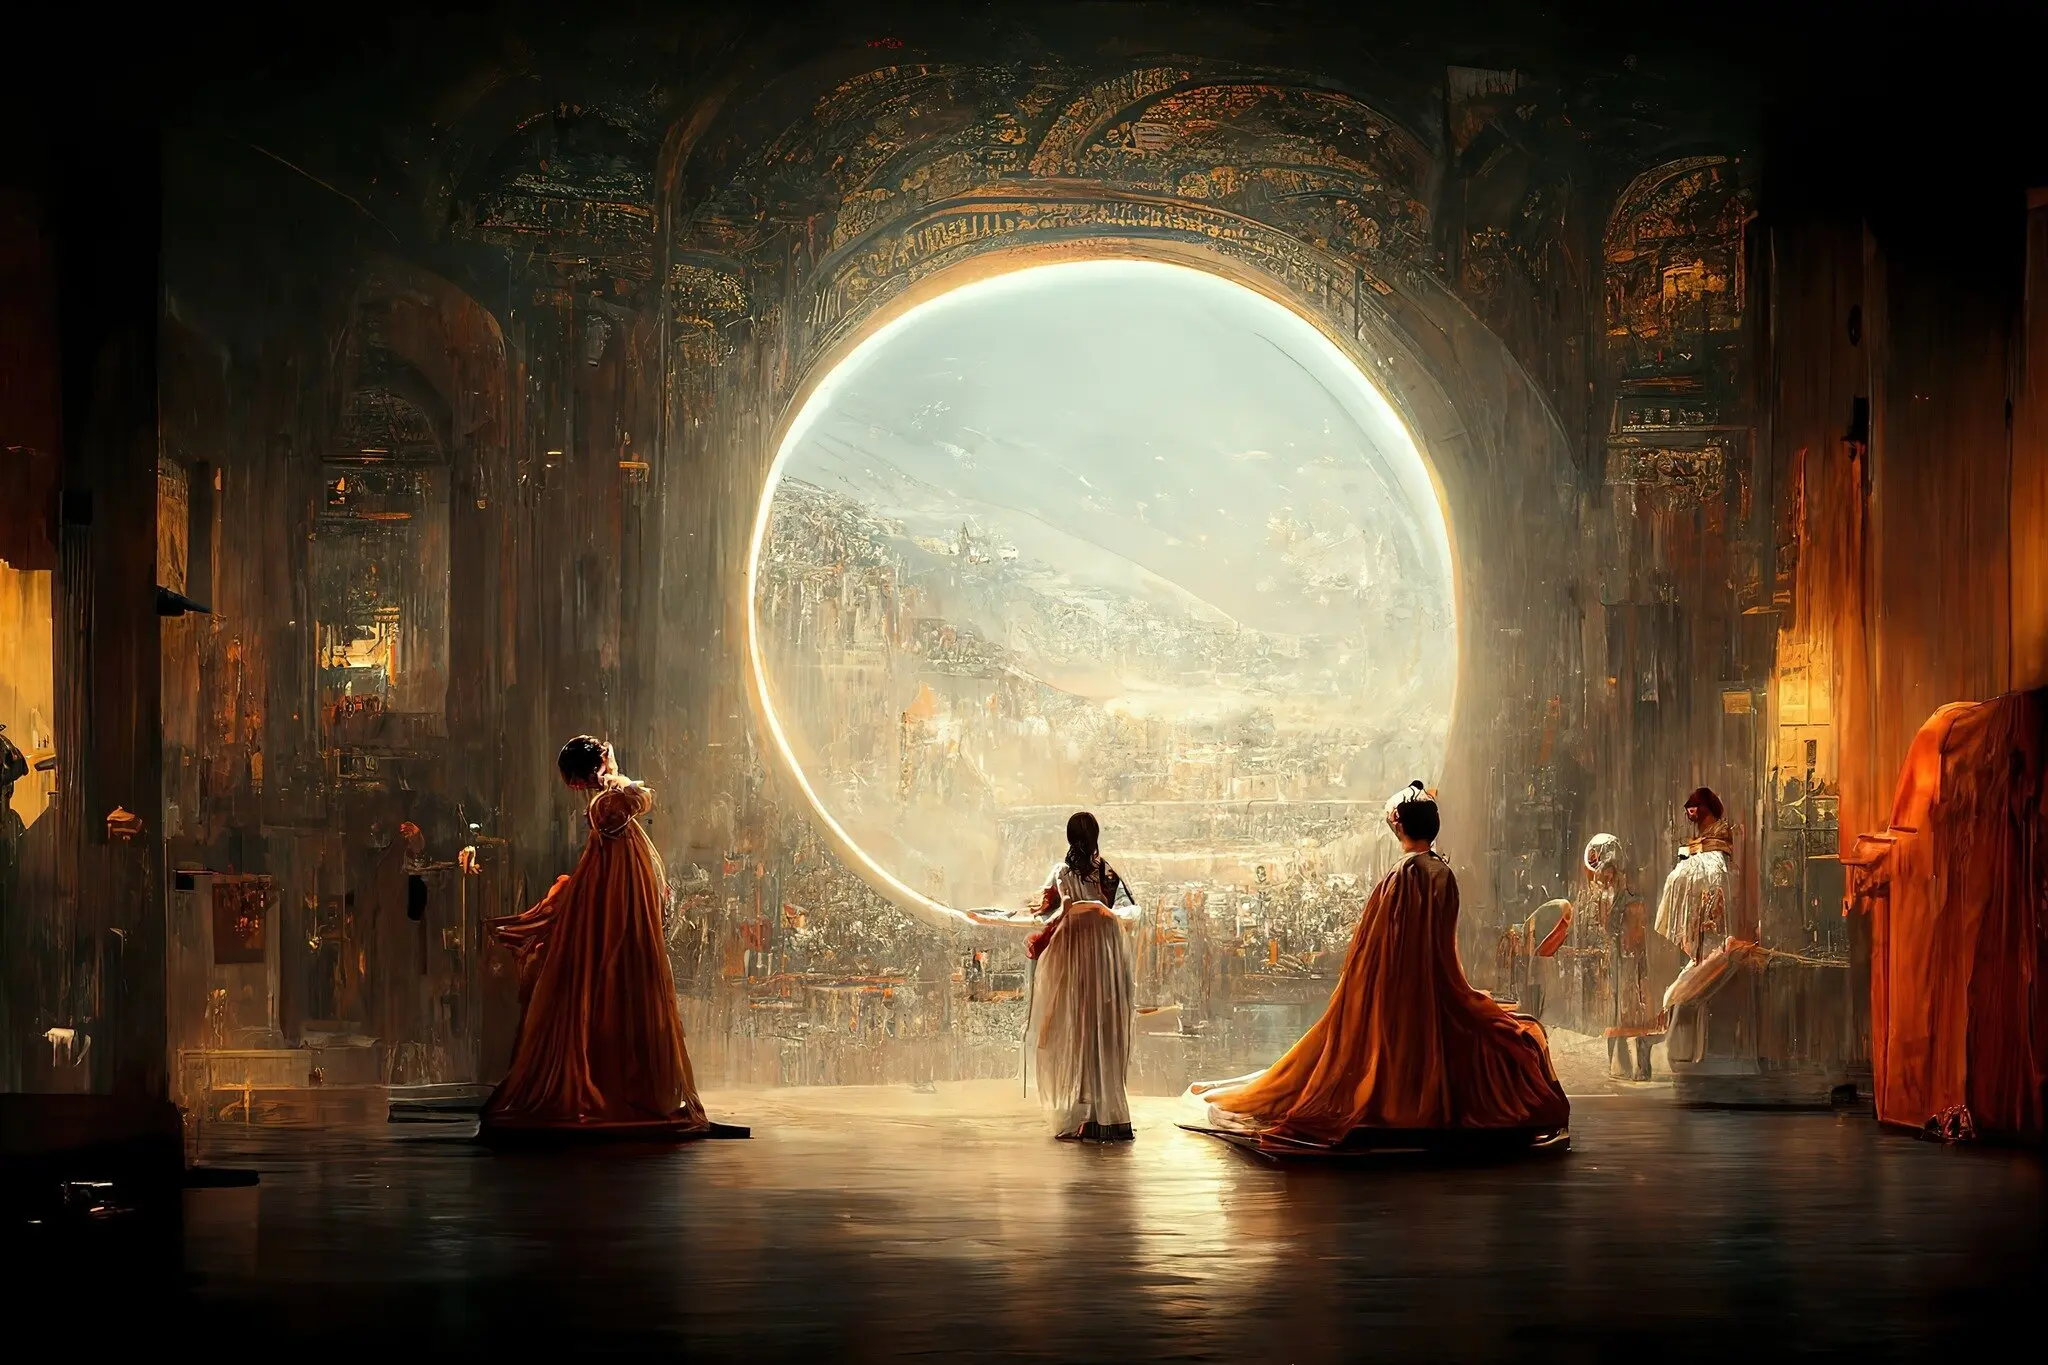
\includegraphics[width=0.78\linewidth]{Images/ColoradoStateFairWinner.png}
			\caption{\tiny “Théâtre D’opéra Spatial”, Winner of the blue ribbon in the fair’s contest for emerging digital artists by Colorado State Fair’s annual art competition}
		\end{figure}
	\end{frame}

\begin{frame}
% - Portrayal of socially unacceptable or midly illegal actions: kid smoking, bullying
% 	-> Is this below the "needs regulation" bar? overregulation?
	\frametitle{Portrayal of racism, misogyny, violence, illegal actions }
		\begin{columns}[c] 
			\begin{column}{0.5\textwidth} % Left column width
				\begin{itemize}
					\setlength\itemsep{2em}
					\item Examples: children smoking, extreme violence
					\item DALLE-2 is proven to have social biases \cite{https://doi.org/10.48550/arxiv.2202.04053}
					\item How much of this could even be regulated?
				\end{itemize}
			\end{column}
			\begin{column}{0.5\textwidth} % Right column width
				\begin{figure}
					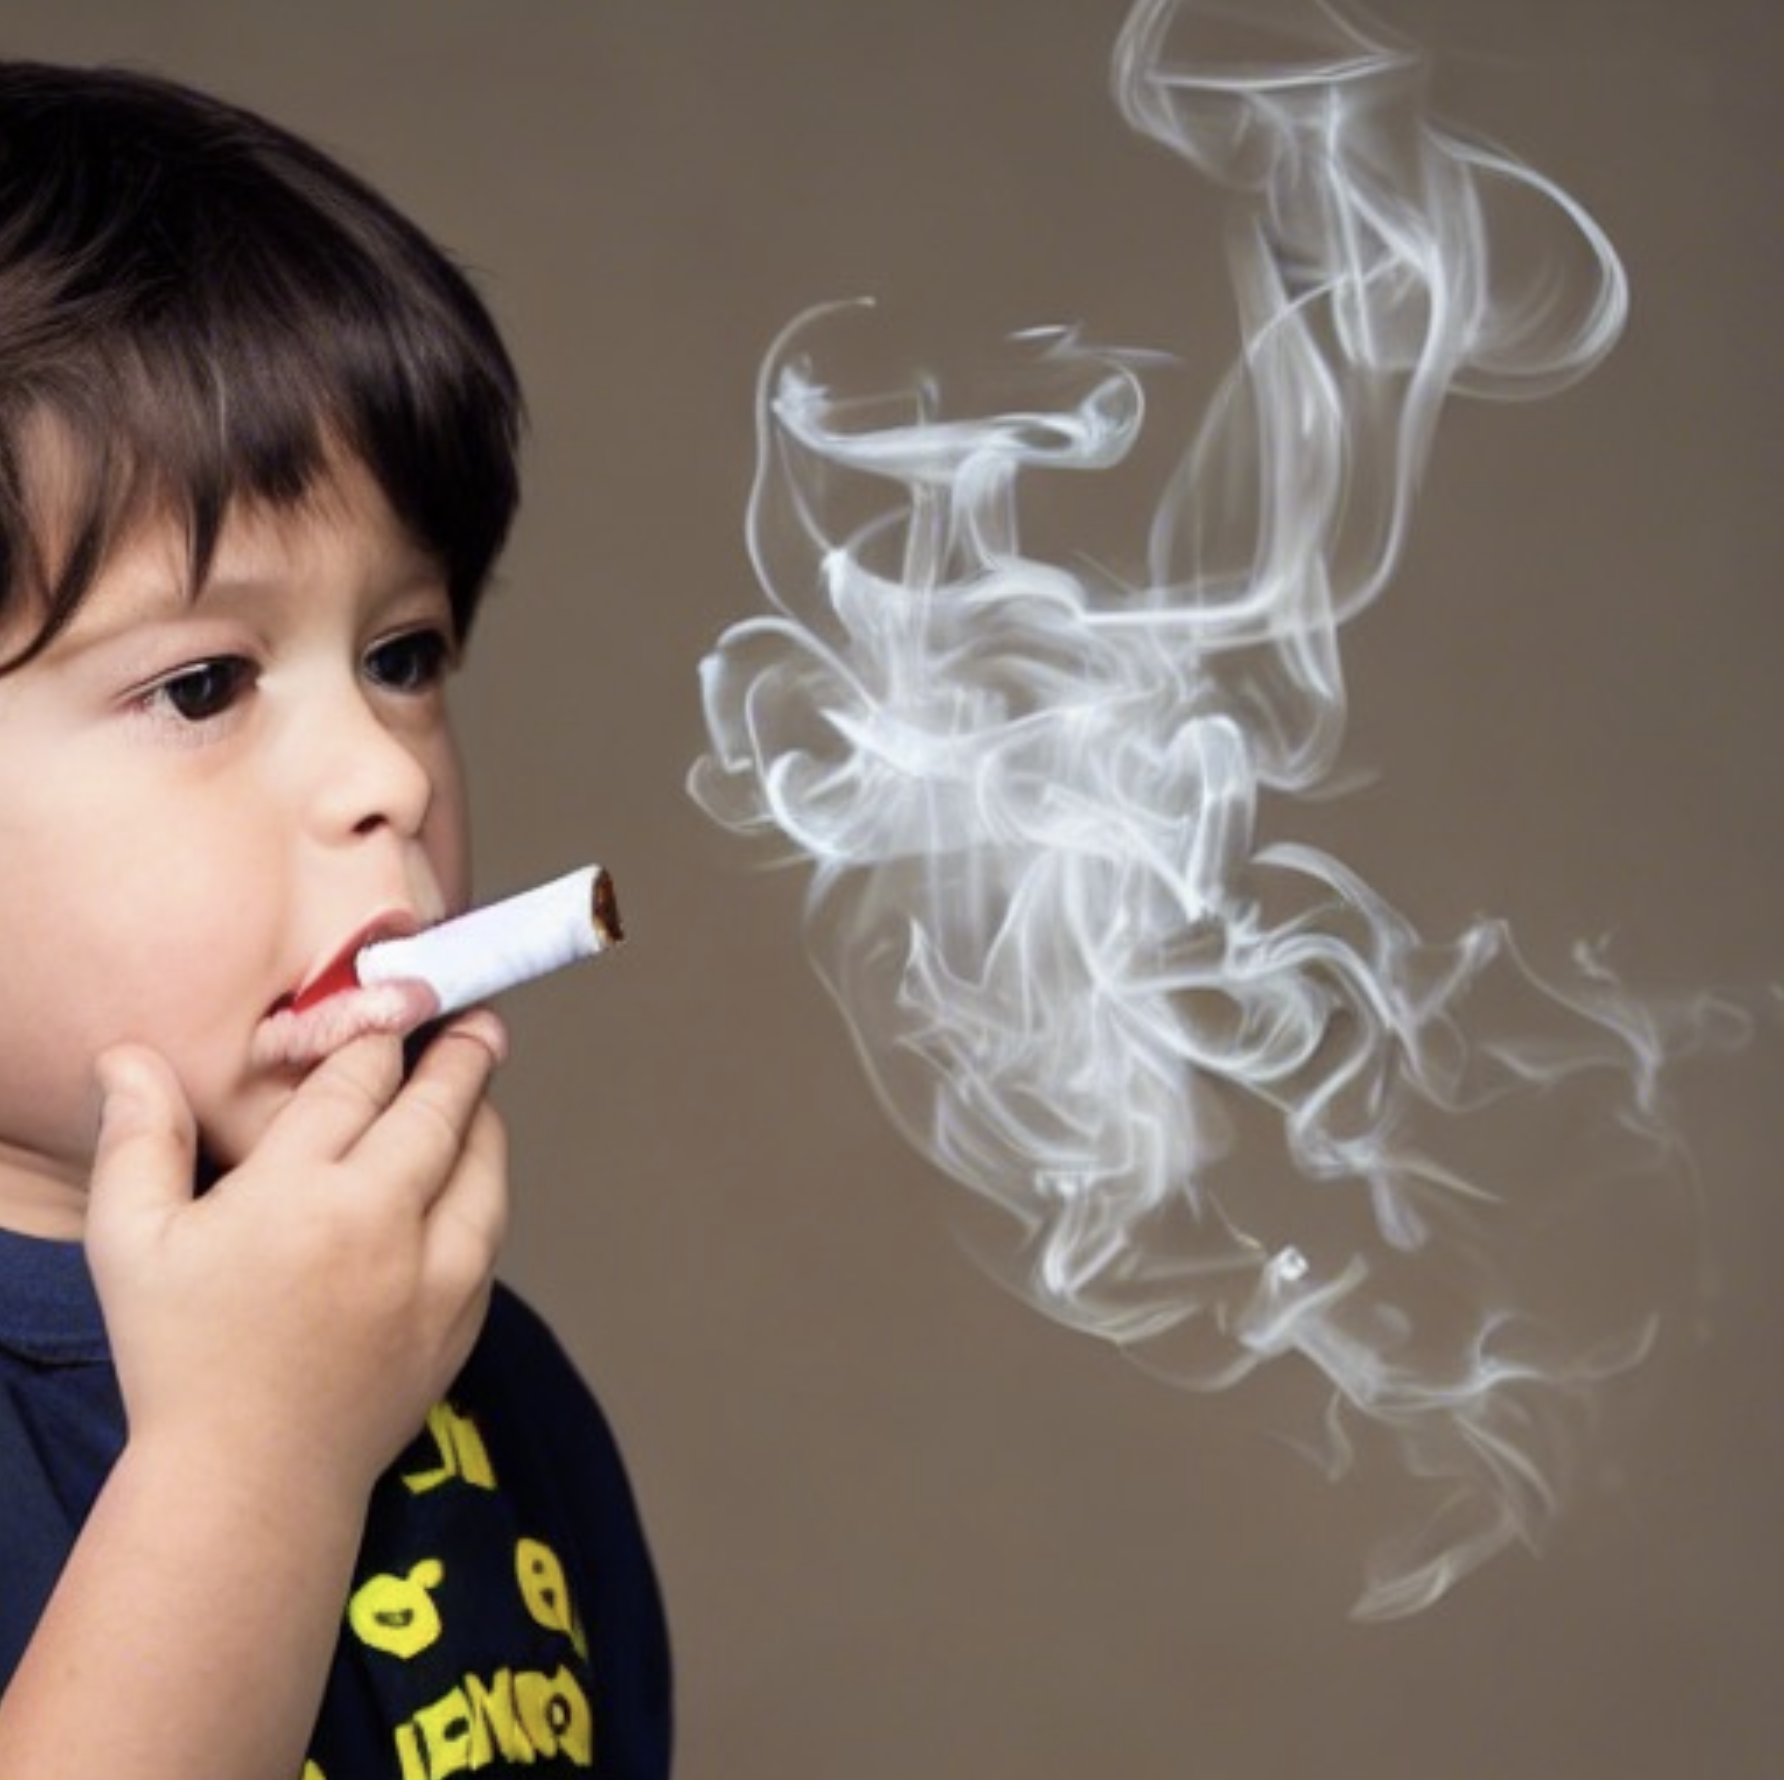
\includegraphics[width=0.5\linewidth]{Images/Ensuring Visual Commonsense Morality for Text-to-Image Generation_kid smoking.png}
					\caption{\tiny A child smoking, generated by Stable Diffusion. Modified from \cite{https://doi.org/10.48550/arxiv.2212.03507}}
				\end{figure}
			\end{column}
		\end{columns}
\end{frame}



\begin{frame}
% - (Child) Pornography
%	-> https://medium.com/mlearning-ai/this-website-can-generate-nsfw-images-with-stable-diffusion-ai-1ee2913de829
% 	-> Child pronography, revenge porn
	\frametitle{Pornography}
	\begin{itemize}
		\setlength\itemsep{2em}
		\item Child pornography
		\item \emph{Un}stable Diffusion: Community targeted specifically at porn generation\cite{UnstableDiffusion}
		\item \textbf{Big risk}, but also a chance for an industry known for bad working conditions?
	\end{itemize}
\end{frame}

\begin{frame}
% - Political Deception
% 	-> depicting political leaders in compromising situations

% https://gnet-research.org/2023/02/17/weapons-of-mass-disruption-artificial-intelligence-and-the-production-of-extremist-propaganda/
	\frametitle{Deception, political propaganda and extremism}
	\begin{itemize}
		\item Lowers the barriers to entry significantly
		\item Propaganda en masse?
	\end{itemize}
	\begin{columns}[c] 
		\begin{column}{0.5\textwidth} % Left column width
			\begin{figure}
				\includegraphics[width=0.6\linewidth]{Images/punkSkinHeadMusicAlbumCover.png}
				\caption{\tiny MidJourneyAI generated punk-skinhead music album cover art, modified from }
			\end{figure}
		\end{column}
		\begin{column}{0.5\textwidth} % Right column width
			\begin{figure}
				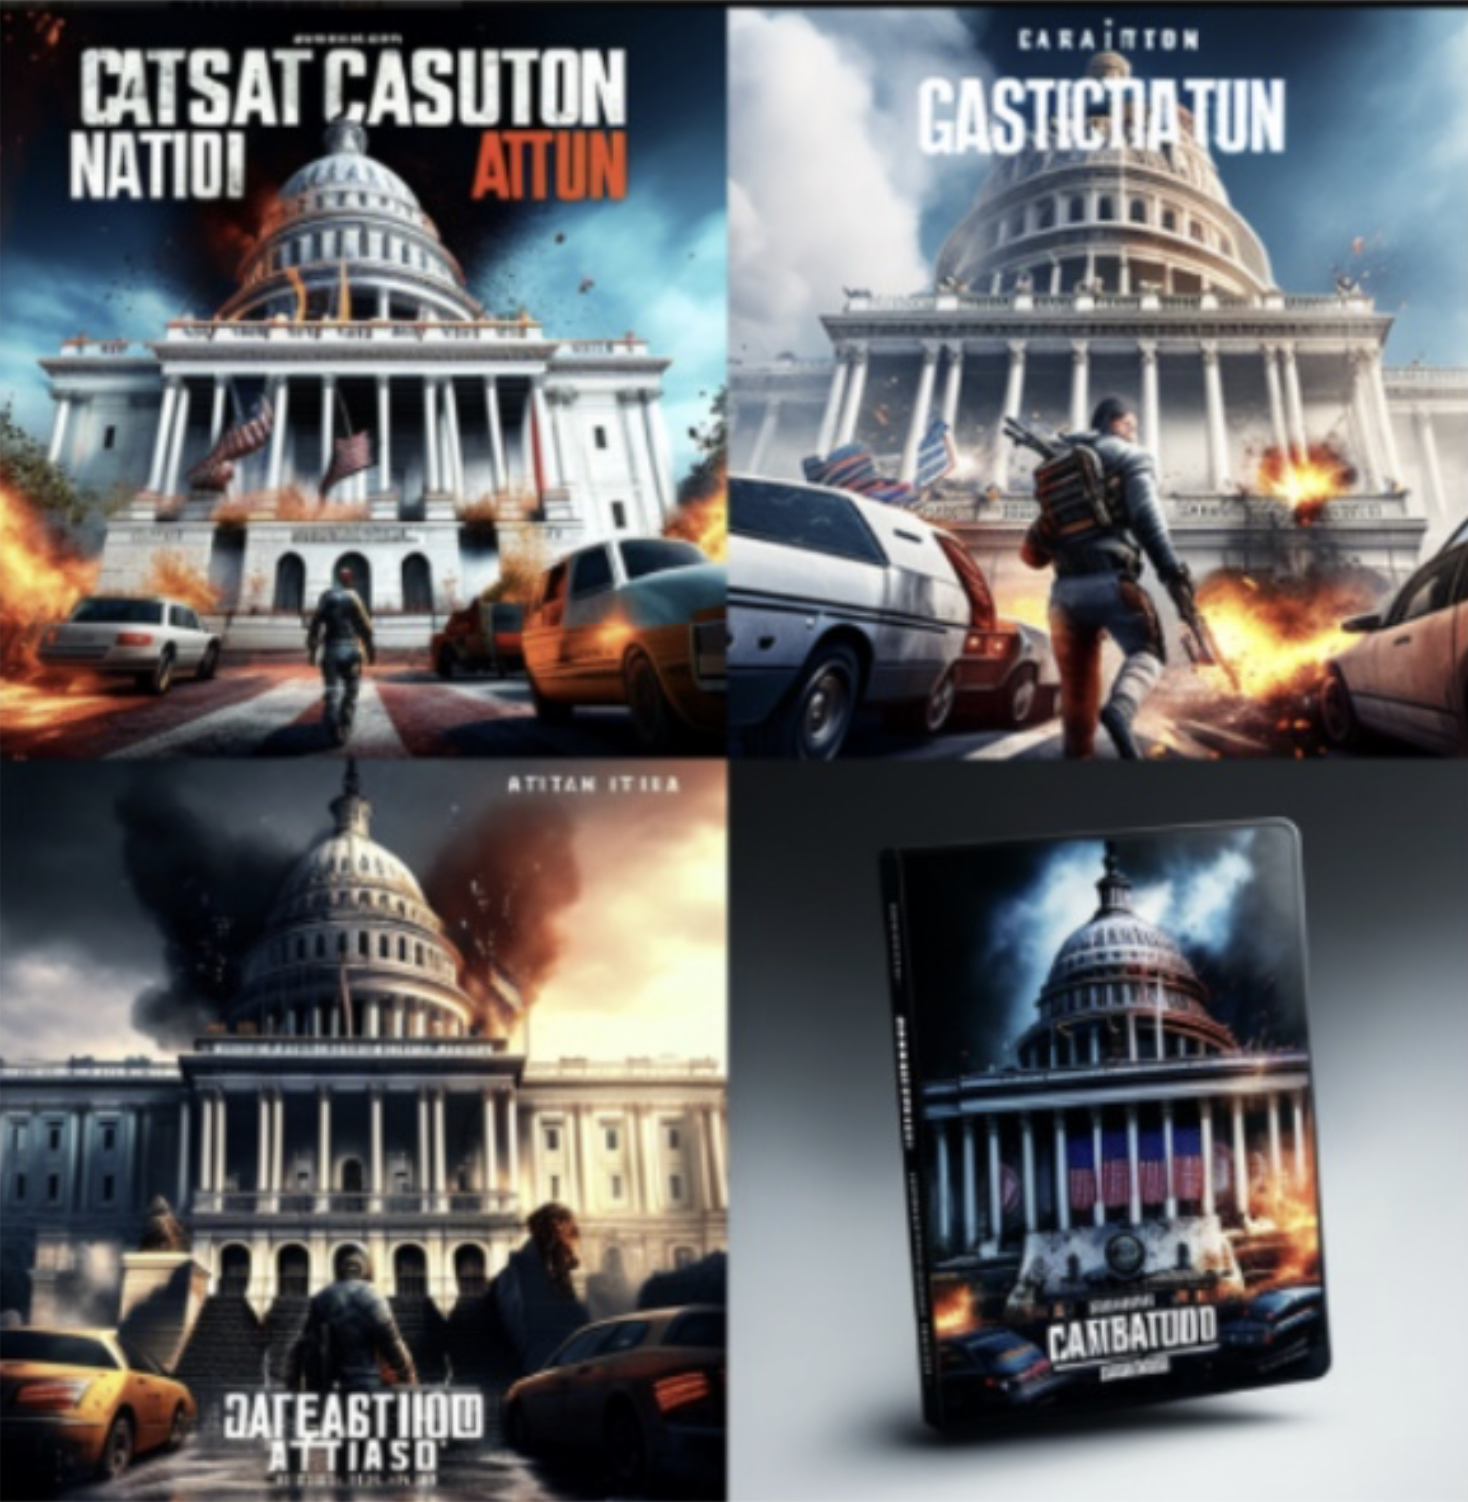
\includegraphics[width=0.6\linewidth]{Images/GameCoverArtCapitolInsurrection.png}
				\caption{\tiny Jan 6. U.S. Capitol insurrection video game art generated by MidJourneyAI, modified from } 
			\end{figure}
		\end{column}
	\end{columns}

\end{frame}



\begin{frame}
	\frametitle{A LOT of potential for misuse!}
	\begin{itemize}
			\item{Highly realistic images of individuals without their consent}
			\item{Portrayal of socially unacceptable actions:}
			\begin{itemize}
			\item{Violence}
			\item{(Child) pornography}
			\item{Racism}
			\item{Artists taking credit for AI-work(?)}
			\item{...}
			\end{itemize}
	\end{itemize}
\end{frame}

\begin{frame}
	\frametitle{What is currently being done?}
	\begin{itemize}
		\setlength\itemsep{2em}
		\item no official regulations
		\item "every man for himself"
	\end{itemize}
\end{frame}

\begin{frame}
	\frametitle{Visualization: some guidelines are strict, some less so}
	\begin{columns}[c] 
		\begin{column}{0.5\textwidth} % Left column width
			\begin{figure}
				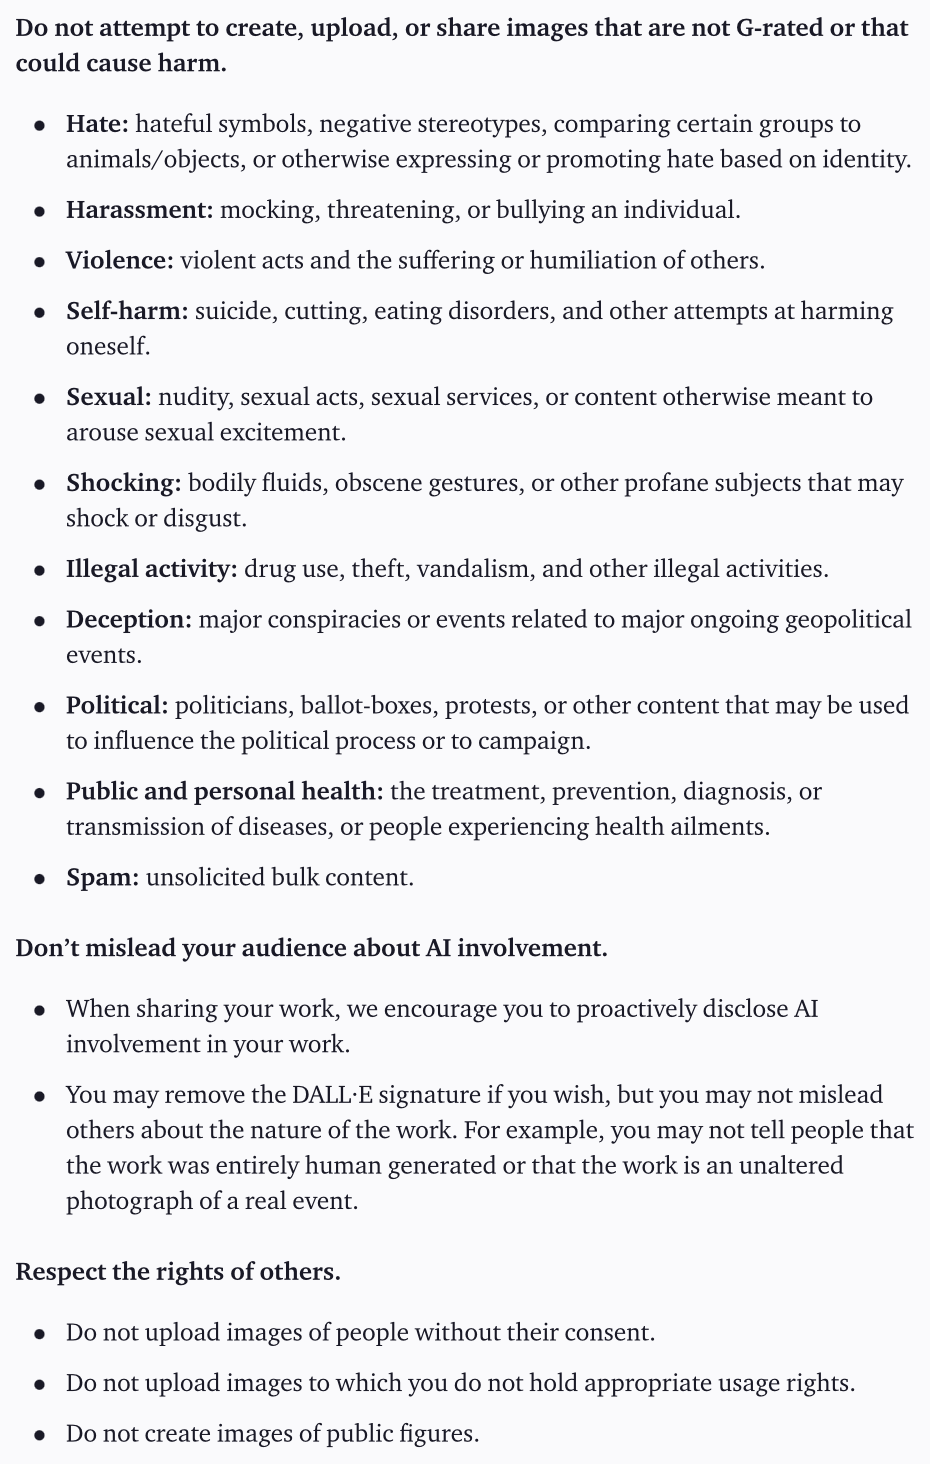
\includegraphics[width=0.60\linewidth]{Images/CommunityGuidelinesDALLE2.png}
				\caption{\tiny Excerpt from the Community Guidelines of OpenAI's Dall-E-2\cite{DallETOS}.}
			\end{figure}
		\end{column}
		\begin{column}{0.5\textwidth} % Right column width
			\begin{figure}
				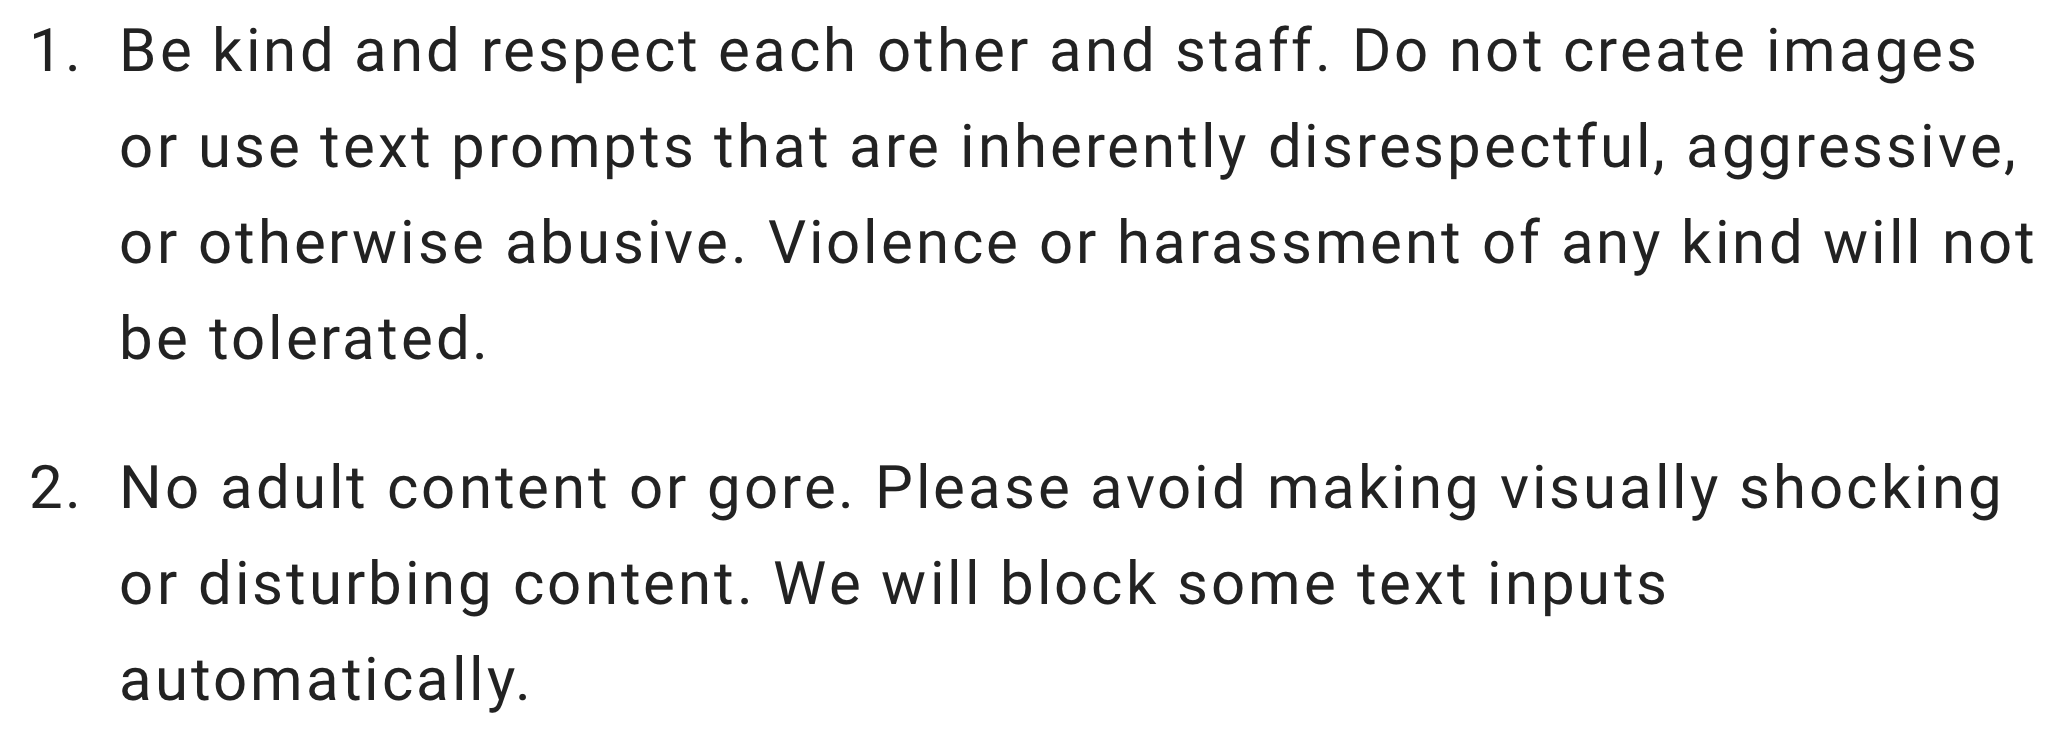
\includegraphics[width=0.60\linewidth]{Images/CommunityGuidelinesMidjourneyAI.png}
				\caption{\tiny Excerpt from the Community  Guidelines of MidJourney Inc's MidjourneyAI\cite{MidJourneyTOS}.} 
			\end{figure}
		\end{column}
	\end{columns}
\end{frame}

\begin{frame}
\begin{center}
	\huge What could be done?
\end{center}
\end{frame}



\begin{frame}
% what can be done against this?
% - add watermark / clear labeling of AI-generated images
% - add content filter ("select keywords, seperate model to detect immorality")
% - restrict who can access models ("driver's license")
% - impose strict limit on training data (if there is no pornography / nudity in the training data, the model wont know to generate related images WELL)
% - legal liability for misuse
% 	-> who is liable? programmer / business / user
	\frametitle{What could be done?}
	\begin{itemize}
		\setlength\itemsep{1em}
		\item Watermarks / Clear labeling of AI-generated images
		\item Content filters
	\end{itemize}

	\begin{figure}
		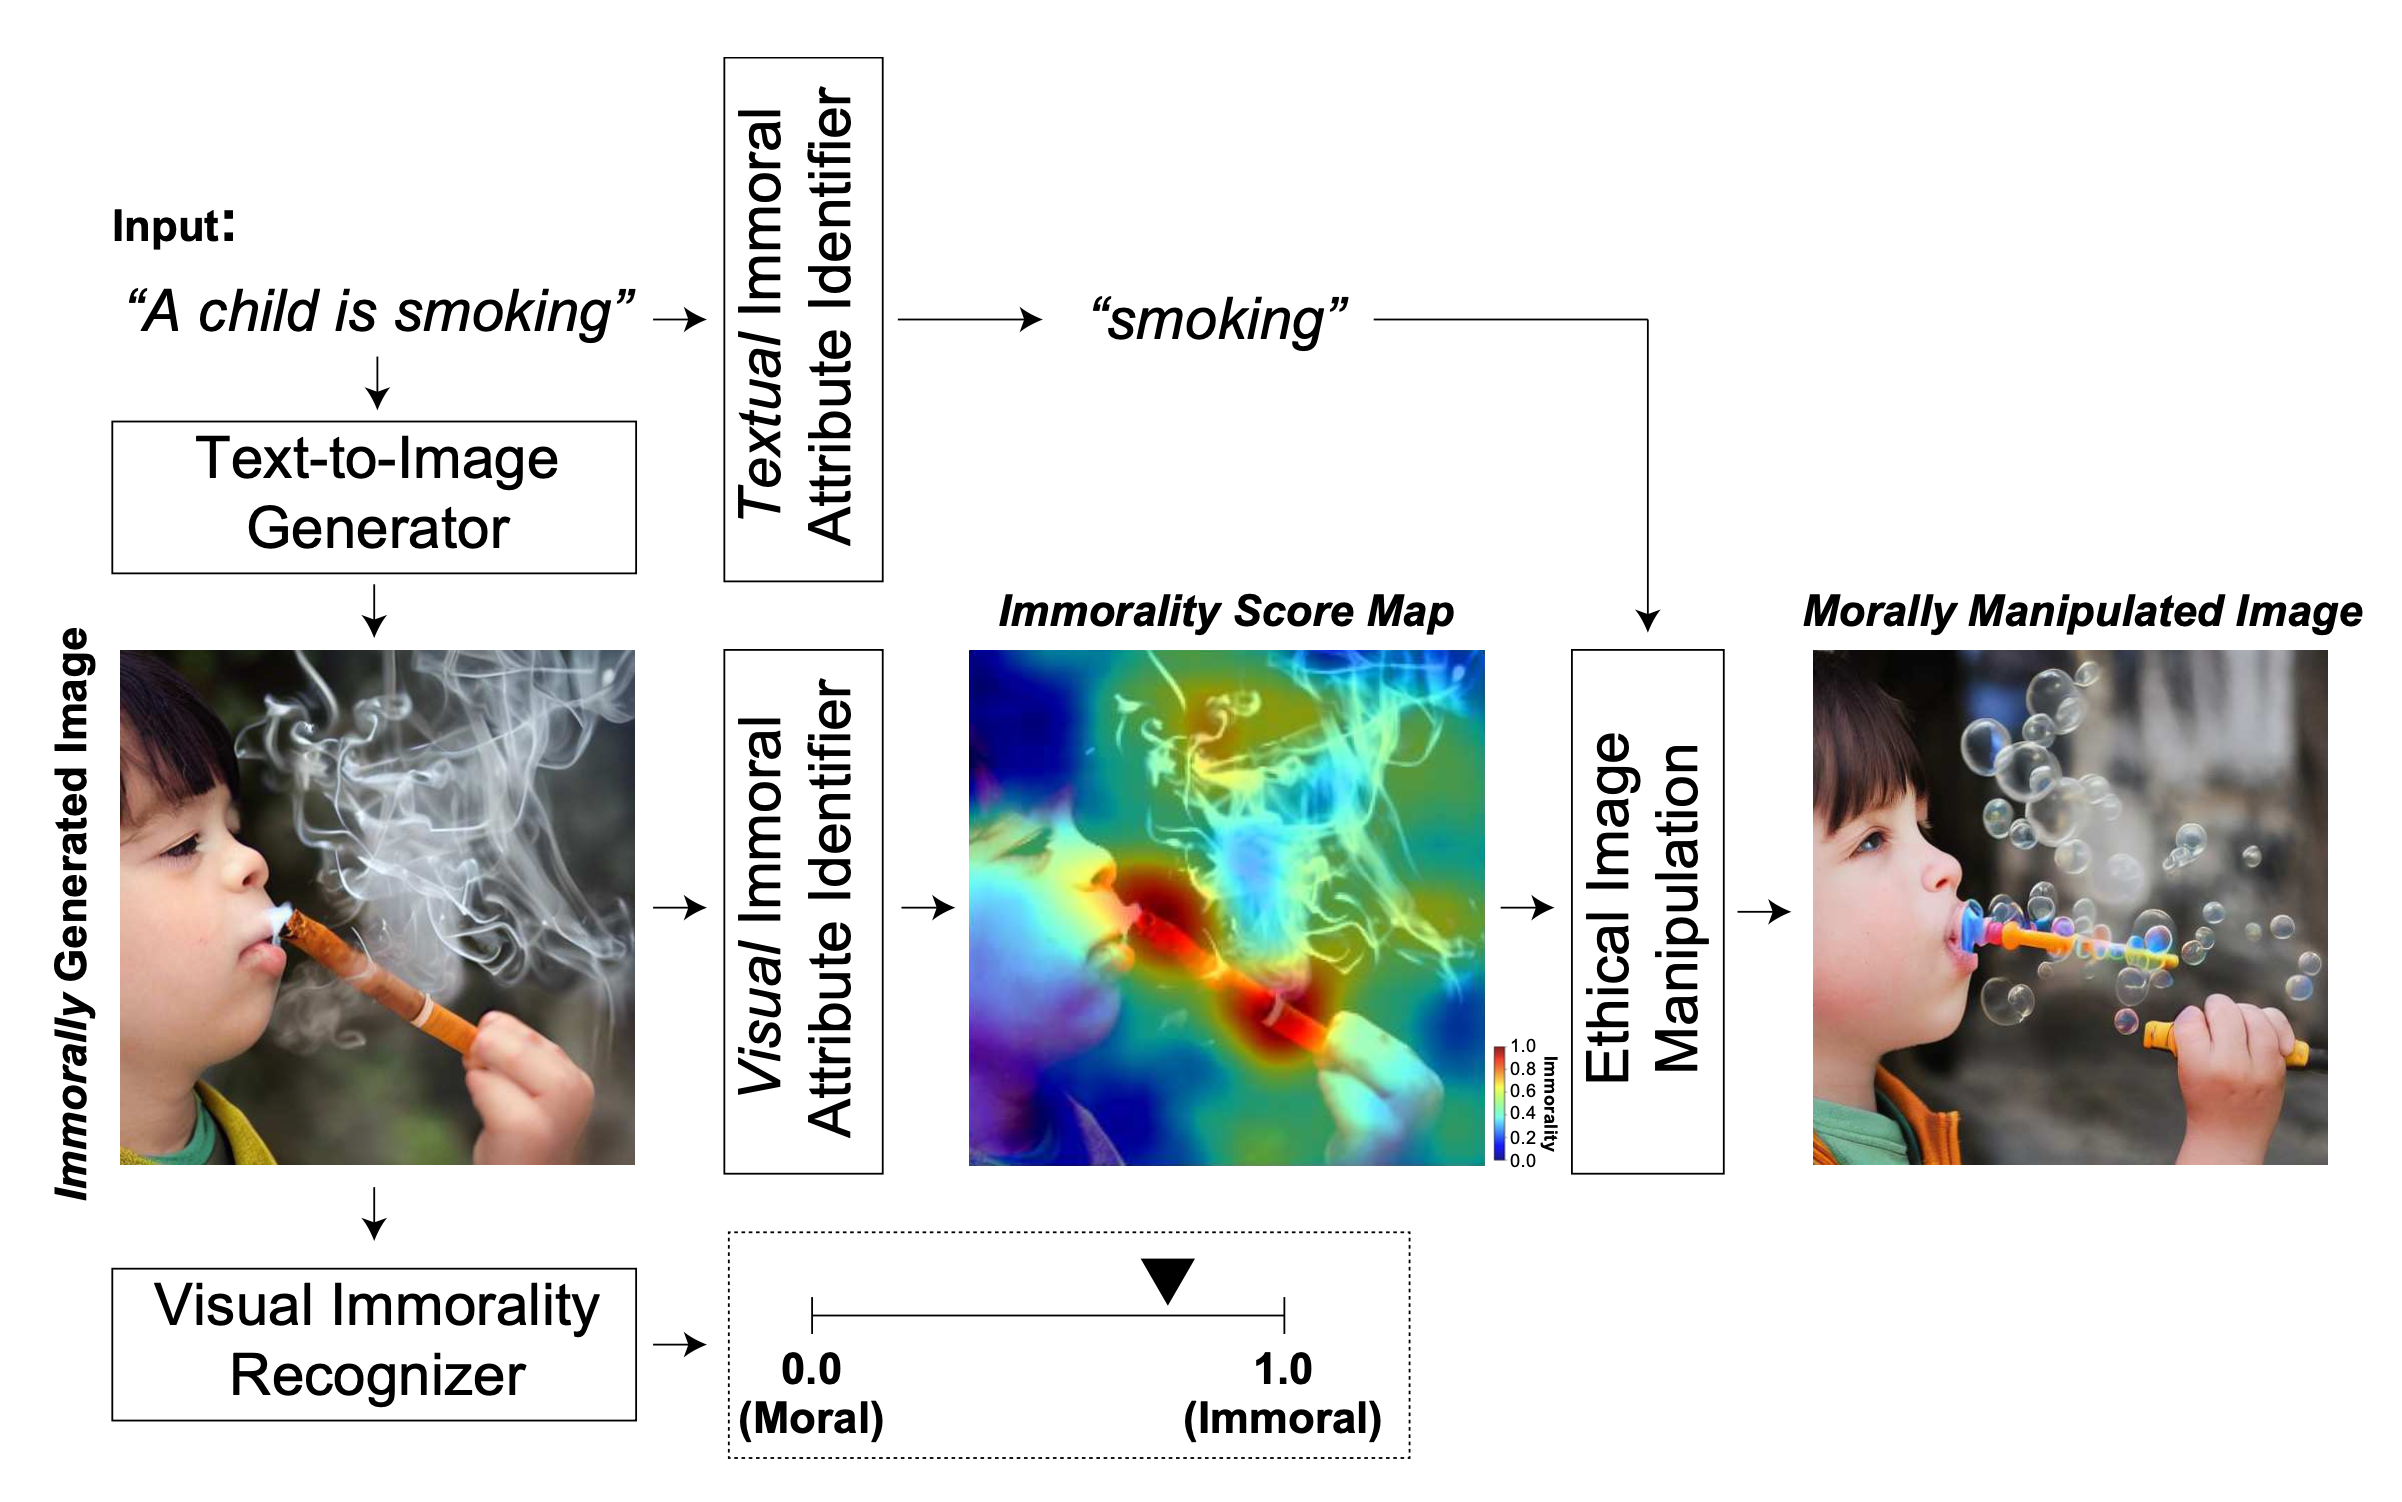
\includegraphics[width=0.7\linewidth]{Images/CommonSenseMoralityCorrection.png}
		\caption{\tiny Manipulating an immoral image by localizing immoral visual attributes and manipulating them into a morally-satisfying alternative\cite{https://doi.org/10.48550/arxiv.2212.03507}.} 
	\end{figure}

\end{frame}

\begin{frame}
	\frametitle{What could be done?}
	\begin{itemize}
		\setlength\itemsep{1em}
		\item Restrict who can access models ("driver's license")
		\item Impose strict limit on training data -> "mischief models"
		\item Establish legal liability for misuse
	\end{itemize}
\end{frame}

\section{Conclusion}


%------------------------------------------------
\begin{frame}[plain]{References} 
    \nocite{*}
	\tiny
    \bibliographystyle{unsrt}
    \bibliography{bib.bib}
\end{frame}


%----------------------------------------------------------------------------------------

\end{document} 